%!TEX root = ../thesis.tex
%*******************************************************************************
%****************************** Second Chapter *********************************
%*******************************************************************************

\chapter{Quantifying received dose errors introduced by modelling approximations in reinforced concrete shielding}
\label{chap:homogenisation}

\ifpdf
    \graphicspath{{Chapter2/Figs/Raster/}{Chapter2/Figs/PDF/}{Chapter2/Figs/}}
\else
    \graphicspath{{Chapter2/Figs/Vector/}{Chapter2/Figs/}}
\fi

% ITER report is robust and actually quite well written, use as base
% Check with Roddy I can use material from this report
% Need some introductory material on spatial homogenisation:
%     Raoul's report?
%     Wider literature
% Additional figures which might be nice:
%     Nice SDDR photon ratio
%     Interpolated (time, E, ratio) heatmap

\section{Outline}
This chapter looks at %%%

%INTRODUCTION
\section{Introduction}
The ITER nuclear fusion experiment will begin DT operation in the 2030s. At 500MW fusion power the source rate of 14.1MeV neutrons will approximately $1.8\times10^{20}$ s\textsuperscript{-1}. For comparison, JET's maximum source rate to date is 30 times less. But the real difference is in the fluence. JET's lifetime neutron budget is $2\times10^{21}$ \cite{Lobel08}, or 10 seconds of operation for ITER-DT. The ITER life-time budget is approximately $3\times10^{27}$ neutrons.

Designing a complex device such as a superconducting tokamak to operate in this radiation environment is a particularly challenging aspect of the ITER project. Care must be taken both to shield sensitive components like semiconductor devices from Single Event Effects (SEE) and to prevent excessive nuclear heating in large systems like the superconducting coils. The high flux and fluence of high energy neutrons means activation in areas like the Neutral Beam (NB) cells and in the Tokamak Cooling Water System (TCWS) will be significant. And of course, gamma from these activated components, and the prompt radiation of a thermonuclear plasma must be shielded against to protect the workforce operating and maintaining the plant.

Quantifying the absorbed dose to radiation sensitive components, or the equivalent dose to personnel requires crafting a computer model of the problem and typically making a series of assumptions and simplifications in the process. For reinforced concrete radiation shields, this often entails either homogenising the rebar with the concrete, or even neglecting the presence of rebar entirely. This process introduces systematic error into the reported solution of the problem. However, uncertainty in an answer is not solely from geometrical simplification, but also from other input data. Cross-section, secondary particle and decay data can be flawed or missing and materials compositions can be incorrect. In the case of reinforced concrete, the water and therefore hydrogen content is uncertain. This is because not only can the water content change from batch to batch, but also over time (during the plant lifetime) for a given batch.

\subsection{Radiation shielding}
% Lit review.

\subsection{Spatial homogenisation}
% Lit review.

\subsection{ITER bioshield}

%METHOD
\section{Method}
The modelling simplification under investigation is that of spatial homogenisation and how it affects doses to workers, whether prompt or delayed. It is theorised that any errors incurred by this modelling approximation will be functions of geometry and material composition. For each set of variables interrogated, at least two simulations will be performed. One will have a high-fidelity model of the real-world problem geometry with reinforcing bar and stirrup rods faithfully reproduced. The other will smear the rebar across the concrete, homogenising the two materials into one with a density equal to the mass weighted sum of the concrete and steel constituents. 

Simulations employing realistic ITER source particle distributions will tally transmitted or `leakage' fluence at the rear of the shielding walls in both cases. This permits comparison between the modelling approximation and the higher-fidelity simulation.

\subsection{Model geometry}
The heterogeneous, realistic wall is constructed of a large concrete block, with two meshes of rebar, one buried below each face. The distance from wall exterior to rebar is known as the cover depth. Connecting the two meshes are a small number of narrow gauge `stirrup' bars. The homogeneous model is the same external dimensions and total mass as the heterogeneous one, but without an internal steel structure and with homogenised materials.

A Python program has been written to take wall depth, cover depth and rebar diameter as input variables to construct a corresponding MCNP model. This model utilises lattices to construct the repeated features of the reinforced concrete wall. The concrete block dimensions are $(x, y, z) = (10, y, 10)$ where $y$ is the wall thickness. Embedded within the block are the major two meshes of steel reinforcement. These meshes are always constructed with 200mm spaced rebar extendeding in both the x and z directions \cite{Perez2014}. The meshes are buried a small cover depth from the two $y$-perpendicular surfaces of the wall. Tying the two meshes together are some thinner `stirrup' bars extending in the y direction, with $\approx 4m^{-2}$ of wall face \cite{Perez2014}. A particular level of reinforcement may be referred to as 16HB200, i.e. 16mm diameter rebar, at 200mm spacing.

Material compositions, wall widths, rebar arrangements and steel fractions have been determined from ITER drawings and specifications for concrete walls in the tokamak building. The work have been conducted with a moderated ITER DT fusion neutron source spectrum. The results should give a good idea of the implications of the homogeneous modelling approximation at ITER but also more generally. 

% column span figure
\begin{figure}[H]
  \figuretitle{Homogenising reinforced concrete}
	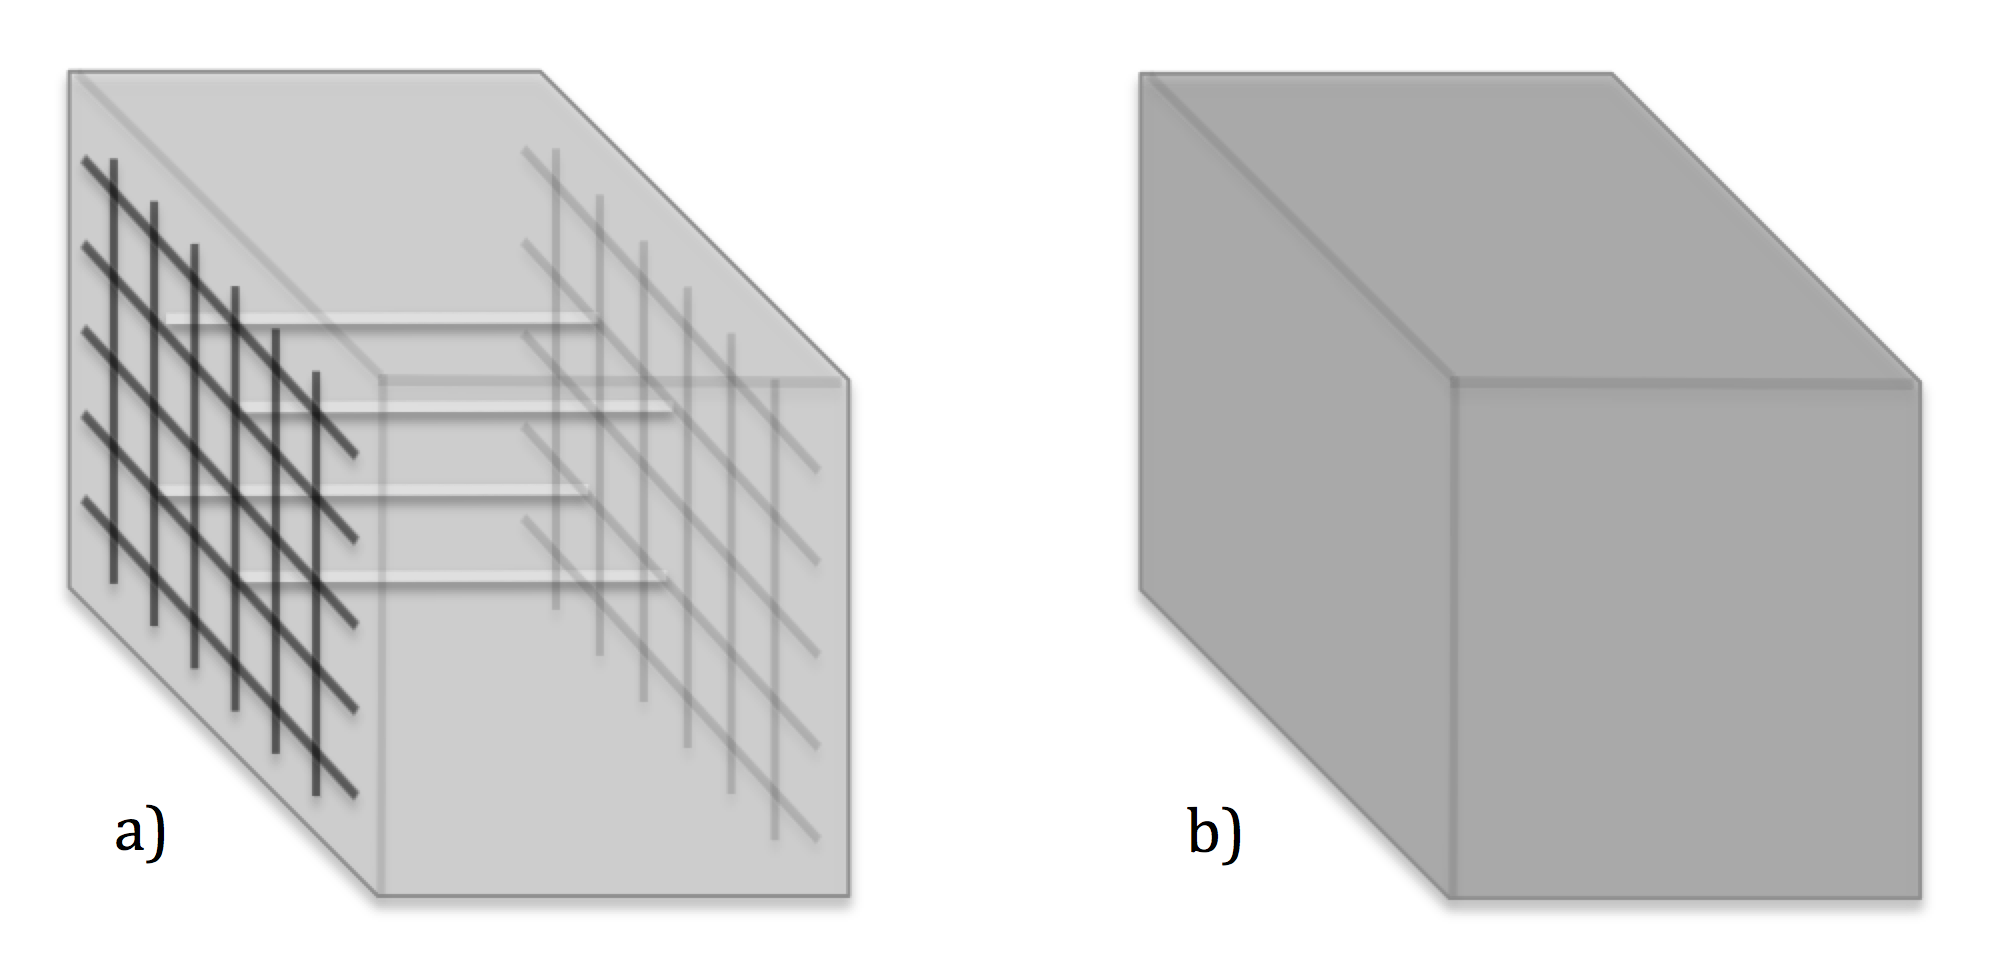
\includegraphics[width=\textwidth]{wall_diagram}
	\caption{The two modelling approaches considered in this investigation. a) Heterogeneous, where the steel reinforcing bar and stirrups are explicitly modelled. b) Homogeneous, where the mass of rebar is 'smeared' through the concrete. The new homogenised material has a greater density than plain concrete, conserving mass.}
	\label{fig:wall_diagram}
\end{figure}

The implications of spatial homogenisation prove to be different for on-load and shut-down (activated) dose rates. It is helpful to consider them seperately. The following two sections detail the methods for determining these two dose rates.

\subsection{Prompt neutron \& gamma radiation}
Determining the dose to personnel beyond a wall requires knowledge of the radiation fluxes there. The on-load gamma flux $\phi_{\gamma}(x,y,z,E,t)$ and neutron flux, $\phi_{n}(x,y,z,E)$, can be computed with Monte Carlo techniques, spawning neutrons from a prerecorded source distribution, $P(x,y,z,E,\Omega)$ at a particular point with a given energy and angle. These particles may propagate through the wall, scattering, being absorbed, exciting nuclei (which later relax through radiative emission) and perhaps leaking out of the back of the shield wall. Tallying this leakage flux of neutrons and photons is the main task of calculating a dose due to radiation.

\subsubsection{Materials}
Although much of the investigation will be by comparing values for homogeneous and heterogeneous responses, it is still important to supply the most accurate input information possible for the simulations. All the compositions that follow were mixed using the PyNE python package \cite{Pyne18} employing natural abundance for isotopic distributions.

\paragraph{Concrete}
The density of concrete used is 2.2g cm\textsuperscript{-3} \cite{Jakhar16}. The composition is shown in table~\ref{tab:concrete}. 

\begin{table}[H]
  \centering
  \begin{tabu} to 0.5\textwidth {X X}
    \toprule
    Element   &   \% weight
    \midrule
    H  &	0.56
    O	 &  49.75
    Na &	1.71
    Mg &	0.26
    Al &	4.69
    Si &	31.47
    S  &	0.13
    K  &	1.92
    Ca &	8.28
    Fe &	1.24
    \bottomrule
  \end{tabu}
  \caption{Concrete composition \% weight from \cite{Jakhar16}. The H content may be overestimated in this mixture. Sampling suggests it may be as low as 0.2\%wt \cite{Aramburu16}. The consequences of such an deviation are substantial and were investigated in work not presented here.}
  \label{tab:concrete}
\end{table}

\paragraph{Steel}
The density of steel used for rebar is 7.85g cm\textsuperscript{-3} \cite{BSsteel05}. The steel minor constituents Cu, Mn, Cr, Mo, V and Ni are not specified in \cite{BSsteel05} however the CEV (Carbon Equivalent Value) is given, a figure for quantitatively comparing the 'weldability' of steels. The CEV formula was used to determine likely \% fractions of the aforementioned elements, giving a material composition as shown in table~\ref{tab:steel}.

\begin{table}[H]
  \centering
  \begin{tabu} to 0.5\textwidth {X X}
    \toprule
    Element   &   \% weight
    \midrule
    Fe	& 97.24
    C   &	0.22
    P   &	0.05
    S   &	0.05
    N   &	0.012
    Mn  &	0.56
    Cr  &	0.16
    Mo  &	0.16
    V   &	0.16
    Ni  &	0.7
    Cu  &	0.7
    \bottomrule
  \end{tabu}
  \caption{Steel composition \% weight from \cite{BSsteel05}.}
  \label{tab:steel}
\end{table}

\subsubsection{Radiation sources}
The effect of spatial homogenisation is considered for both neutron and photon radiation, hence likely distributions are required for both particle types.

No particle direction information was available, so it was assumed that all particles are born travelling perpendicular to the radiation shield. It was reasoned that this is a conservative assumption, liable to increase the discrepancy between heterogeneous and homogeneous approaches as the heterogeneous model has features (the stirrup bars) which are aligned with this initial particle direction.

\paragraph{Neutron}
The neutron source spectrum was obtained in previous work by \citeauthor{Jakhar16} and is shown below as \ref{fig:src_spectra}. The location tallied for this particle spectrum was behind a ITER neutral beam assembly, of neutrons incident upon the shield wall behind. In the ITER plant this area will receive an elevated flux over other areas of the bioshield due to the penetrations from neutral beam injectors into the plasma chamber.

It was provided in the 175 VITAMIN-J group structure. Unfortunately this group structure provides very little information about the fine structure of the thermal neutron distribution below 0.1 eV. This is a deficiency in this study as the source spectrum is heavily thermalised. 

% column span figure
\begin{figure}[H]
  \figuretitle{Neutron source spectrum}
	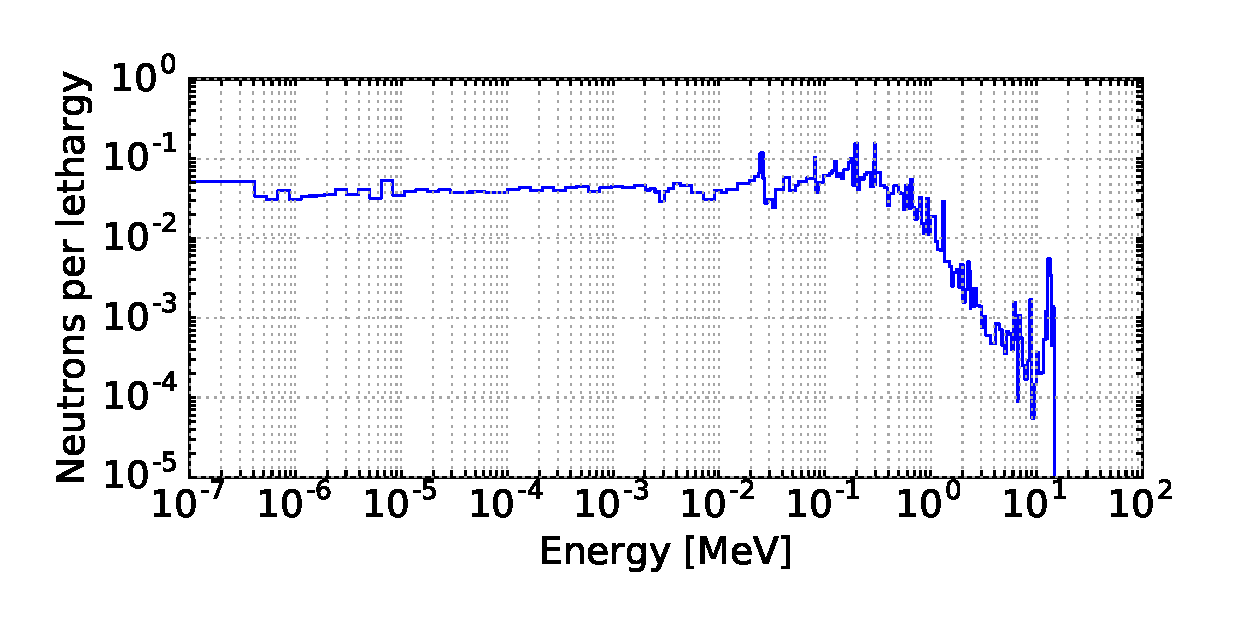
\includegraphics[width=\textwidth]{src_spectra}
	\caption{Neutron spectra for incident radiation. This spectra was tallied at back of the ITER Neutral Beam assembly.}
	\label{fig:src_spectra}
\end{figure}

\paragraph{Photon}
The Tokamak Cooling Water System (TCWS) will move large quantities of water through an intense neutron flux during ITER's operation. This water leaves the tokamak through a network of penetrations and pipes in the surrounding facility. The water is activated mainly by the following reactions: \textsuperscript{16}O(n,p)\textsuperscript{16}N and \textsuperscript{17}O(n,p)\textsuperscript{17}N. These nitrogen isotopes rapidly decay as shown in table~\ref{tab:nitrogen_decay}.

\begin{table}[H]
  \centering
  \begin{tabu} to 0.5\textwidth {X[2] X X X[2]}
    \toprule
    Activation product  & t$_{\frac{1}{2}}$(s)  & Decay mode  & Energy (MeV) [branching ratio \%]
    \midrule
    \textsuperscript{16}N & 7.13  & $\gamma$              & 6.129 [67], 7.115 [5] 
    \textsuperscript{17}N & 4.14  & $\beta \rightarrow n$ & 0.383 [35], 1.171 [53]
    \bottomrule
  \end{tabu}
  \caption{The type, energy and likelihood of decay from activated N isotopes in the ITER water cooling system.}
  \label{tab:nitrogen_decay}
\end{table}

The gamma decay of \textsuperscript{16}N is utilised as a source for several of the simulations presented in section~\ref{subsec:prompt}.

\subsubsection{Computation}
The nuclear data employed was the continuous energy Joint Evaluated Fission and Fusion file 3.2 (JEFF3.2) for neutron transport and MCPLIB84 for photon transport. Radiation transport was conducted with MCNP6v1.0. The MCNP relative error, $R = \frac{\sigma_{s}}{\mu_{s}}$ which is the ratio of sample standard deviation to sample mean was kept to below 0.1 for all energy bins and mesh voxels.

% column span figure
\begin{figure}[H]
  \figuretitle{ICRP74 flux to dose factors}
	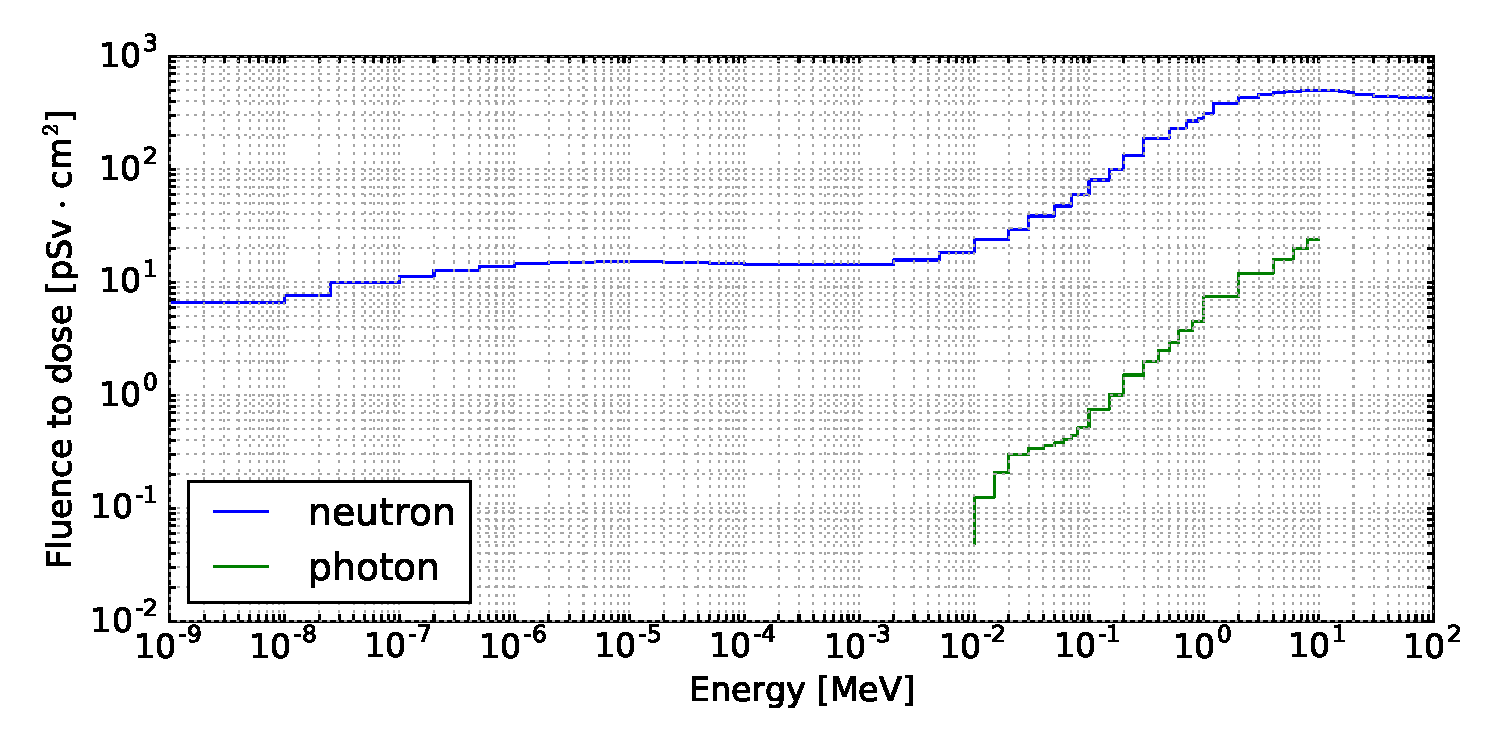
\includegraphics[width=\textwidth]{icrp74}
	\caption{The flux to dose conversion factors for neutron and photon exposure.}
	\label{fig:icrp74}
\end{figure}

The effective dose to humans is a function of the energy and type of radiation. It takes into account the varying susceptibilities of different tissues in the human body. For radiation protection, this is the typical figure quoted when specifying a dose rate. Translation from fluence or flux is by a table similar to that plotted as figure \ref{fig:icrp74}.

%\begin{equation}
%\lambda_{D(e)}=\sqrt{ \frac{ \varepsilon_0 k_B T_{(e)}}{e^2 n_\infty}}
%\end{equation}

\subsection{Shut Down Dose Rate (SDDR)}
The calculation of $\phi_{\gamma}(x,y,z,E,t)$ where $t$ is some time after cessation of plasma operation comprises three main steps:
\begin{enumerate}
  \item 1) Neutron transport---as previously, compute the neutron flux during plasma operation, $\phi_{n}(x,y,z,E)$, recording the neutron flux binned by energy over a spatial mesh. 
  \item 2) Activation---determine the appropriate irradiation scenario, then activate and transmutate the materials present in the problem geometry. 
  \item 3) Photon transport---using the distributed decay gamma source produced by step 2), conduct a radiation transport run to determine the photon flux, $\phi_{\gamma}(x,y,z,E,t)$, converting to effective dose as required.
\end{enumerate}

\subsubsection{Materials}
For analysis of the SDDR, where small impurities can have large contributions to the dose rate, the steel composition was refined \cite{Barabash16}. ITER limits for Co and Ni were imposed, 0.01\%wt and 0.05\%wt respectively. The resulting composition for steel is shown as table~\ref{tab:sddr_steel}.

\begin{table}[H]
  \centering
  \begin{tabu} to 0.5\textwidth {X X}
    \toprule
    Element   &   \% weight
    \midrule
    Fe  &	97.613
    C   &	0.22
    P   &	0.05
    S   &	0.05
    N   &	0.012
    Mn  &	1.08
    Cr  &	0.1
    Mo  &	0.01
    V   &	0.005
    Ni  &	0.05
    Cu  &	0.8
    Co  &	0.01
    \bottomrule
  \end{tabu}
  \caption{}
  \label{tab:sddr_steel}
\end{table}

\subsubsection{Computation}
As for before, radiation transport was conducted with MCNP6 v1.0. Neutron spectra were tallied on a mesh in the shield models. These spectra were used as input to the MCR2S activation linker code \cite{Eade2015}. This program uses these spectra and a corresponding irradiation scenario to compute material changes within the meshed model. These new materials and decay information can be used to generate a photon source from the activated nuclides. The final steps in the calculation are to perform photon transport calculations from the activated wall to a target. The generation of photon sources and transport of emitted $\gamma$-rays must be computed for each decay time step of interest.

In this study the 

was conducted with the FISPACT-II code and EAF2010 nuclear data. The irradiation scenario employed for the activation step was ITER's SA-2, which gives a good representation of the ITER experimental programme total fluence and of the final, end-of-life pulses.

%\end{multicols}

%%%%%%%%%%%%%%%%%%%%%%%%%%
% RESULTS AND DISCUSSION %
%%%%%%%%%%%%%%%%%%%%%%%%%%
\section{Results \& discussion}
%\begin{multicols}{2}

\subsection{Transmission of prompt radiation}
\label{subsec:prompt}
The leakage neutron spectra for a thick (2.1m) concrete wall is shown below as figure \ref{fig:trans_neutron_spec}. The flux has been severely reduced by its interaction with the wall, decreasing from the source by an order of magnitude each 20cm traversed.\par
The reduced thermal flux in the homogeneous case is in part because steel is now available for neutron interactions throughout the depth of the wall. Steel has a greater combined capture cross-section than concrete (radiative capture shown in figure \ref{fig:n_rad_capture}), this acts as a neutron sink. 

% column span figure
\begin{figure}[H]
  \figuretitle{Transmitted neutron spectra}
	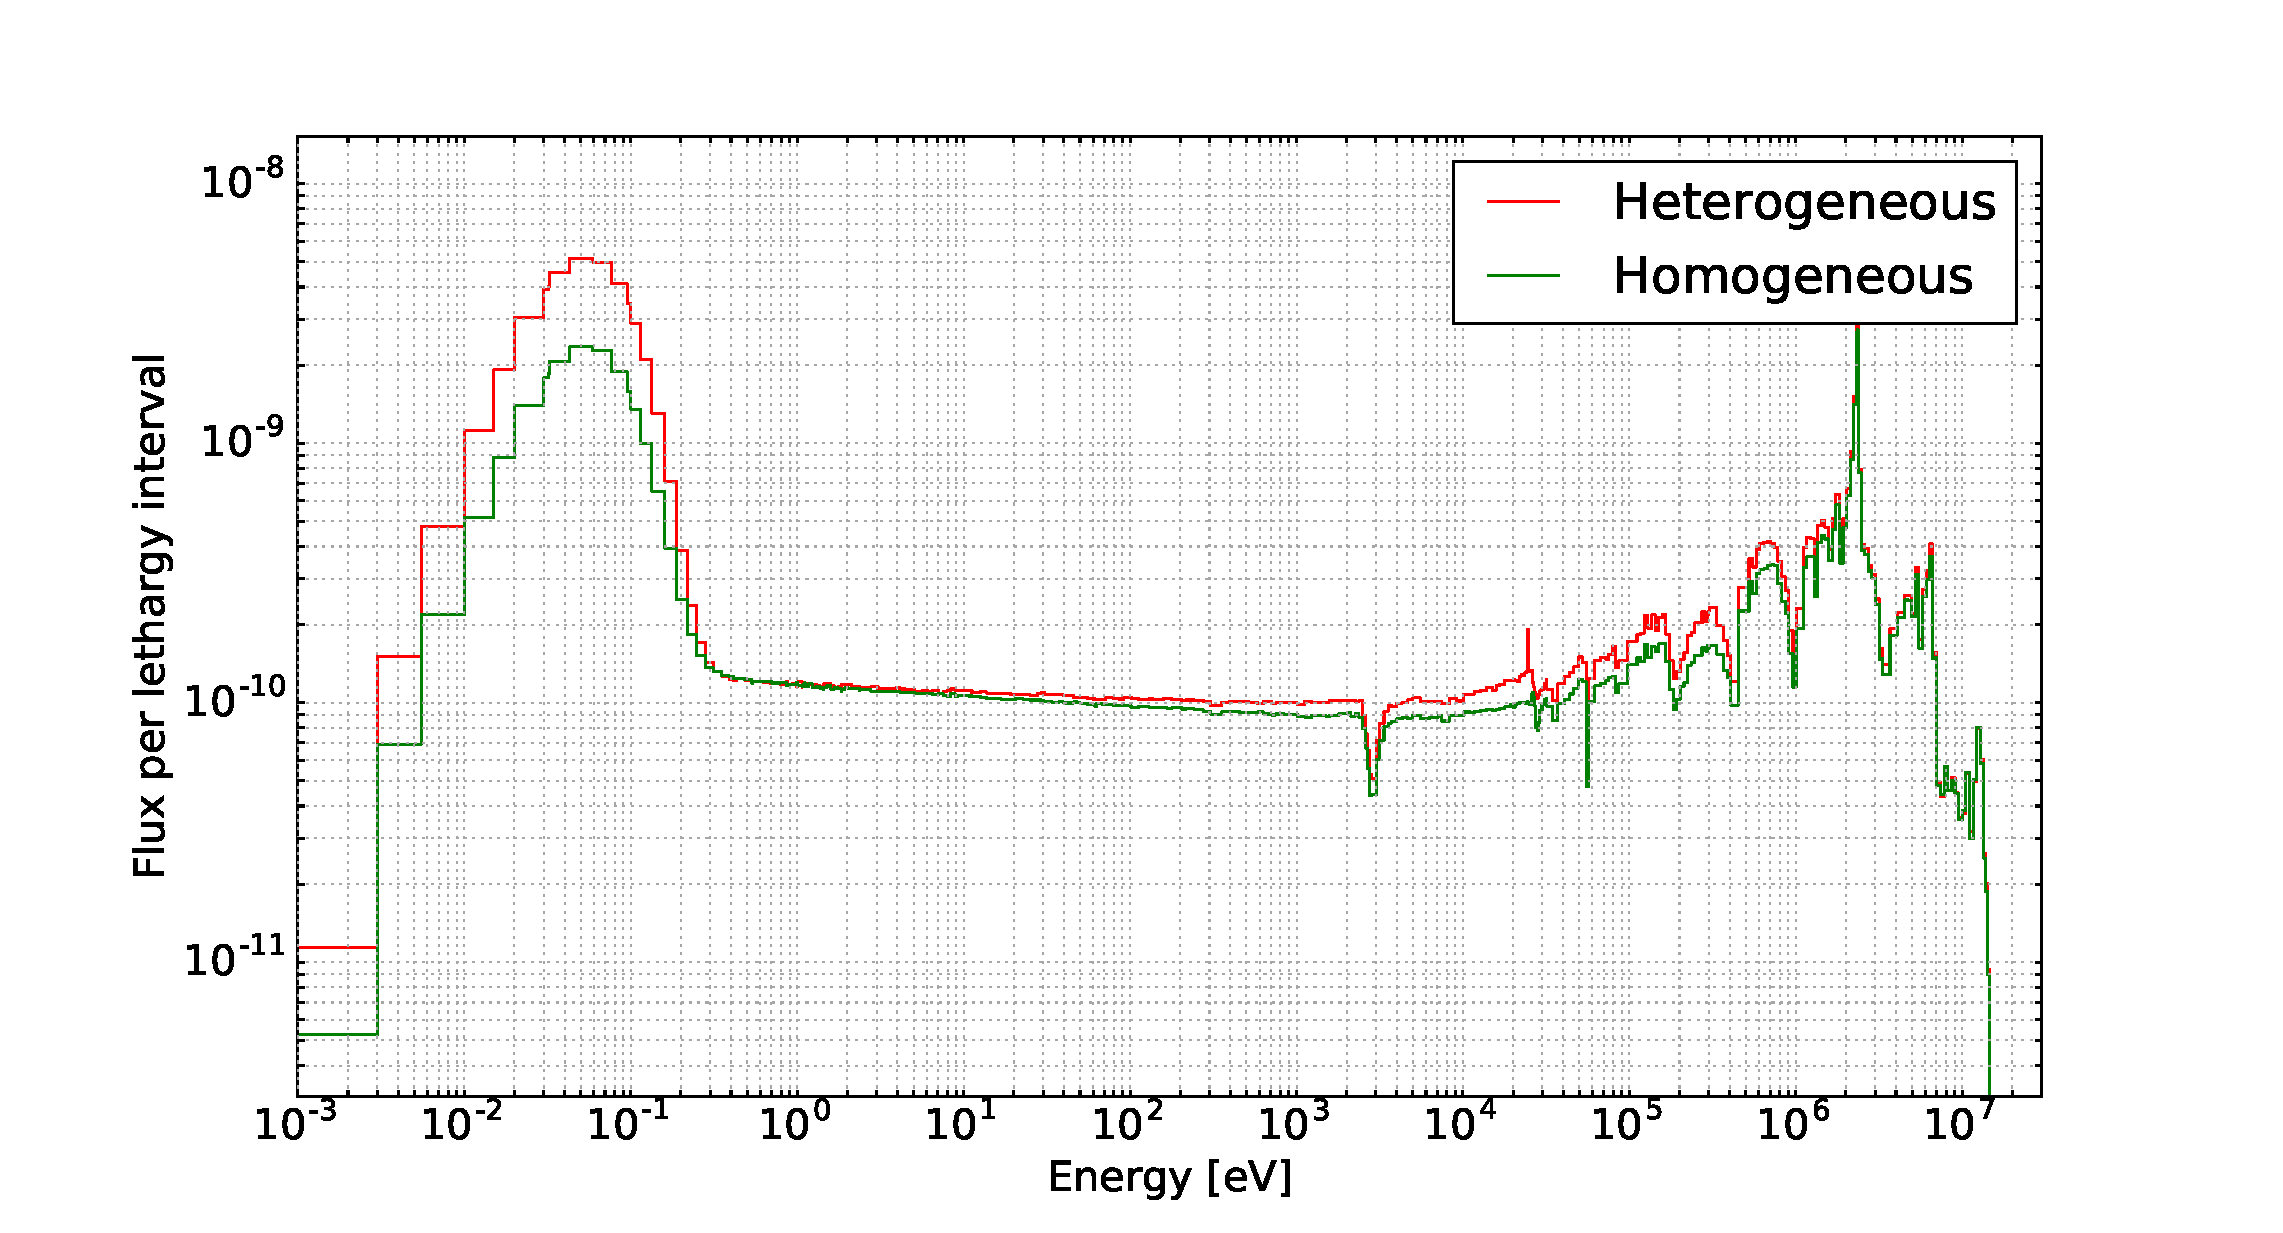
\includegraphics[width=\textwidth]{transmitted_neutron_spectra}
	\caption{The neutron spectra leaving the shield for the heterogeneous and homogeneously modelled cases. Note the substantially reduced thermal flux in the homogeneous simulation. This spectrum has been binned with a finer energy grid than the source, the TRIPOLI 315 group structure.}
	\label{fig:trans_neutron_spec}
\end{figure}

% column span figure
\begin{figure}[H]
  \figuretitle{Radiative capture probability}
  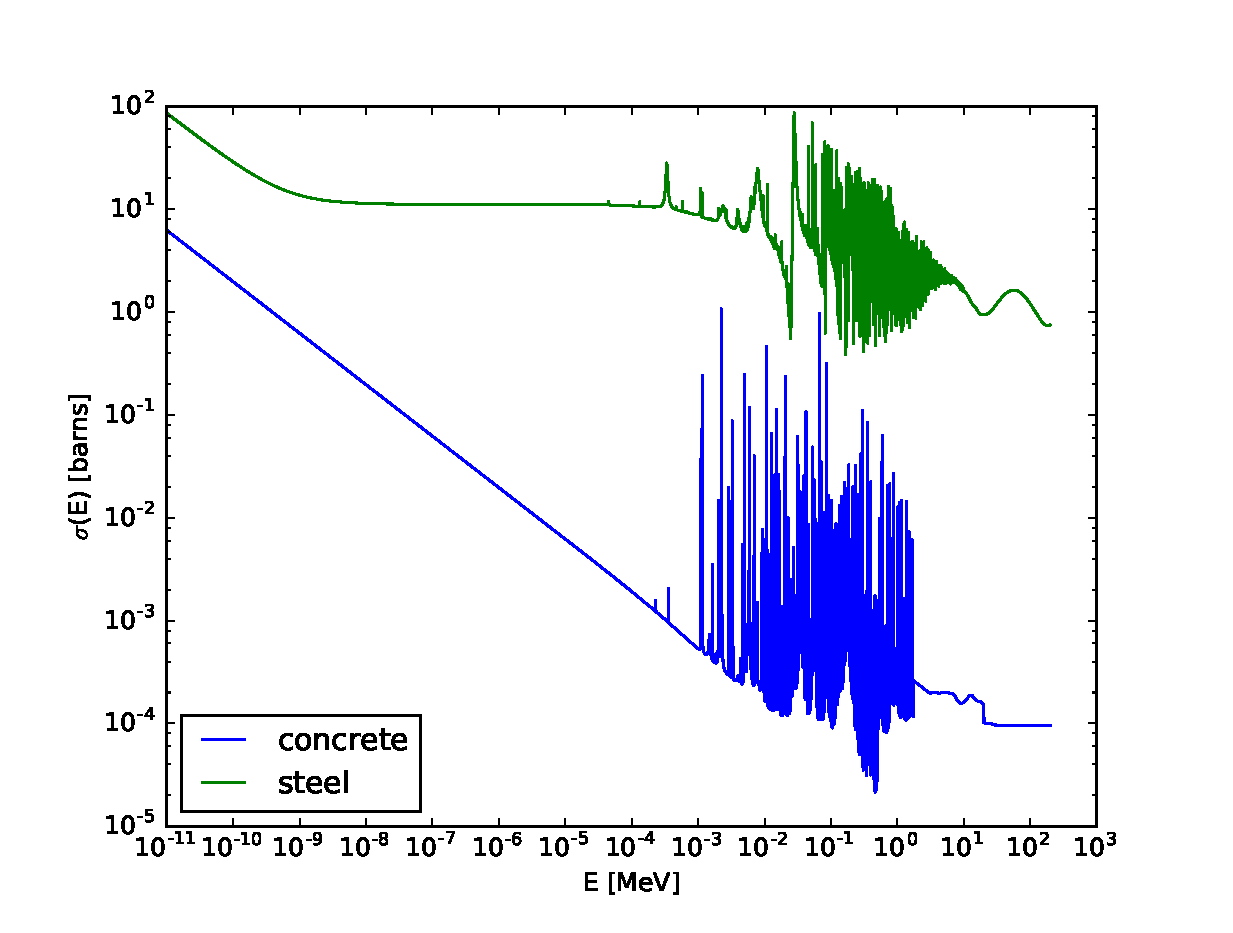
\includegraphics[width=\textwidth]{n_rad_capture}
  \caption{The nuclear properties of steel and concrete are substantially different. Shown here is the cross-section for $(n,\gamma)$ in both materials.}
  \label{fig:n_rad_capture}
\end{figure}

Plotting the ration of the leakage neutron spectra as figure \ref{fig:relative_neutron_spectra} we can see the differences more easily. Thermal flux is underestimated by more than a factor 2. But also, fast flux in the 1keV--1MeV range is underestimated by $\sim1.2$. The fast flux discrepancy is correlated with wall thickness and is negligible for thin (\textless 1m) walls.

% column span figure
\begin{figure}[H]
  \figuretitle{Relative neutron spectra}
	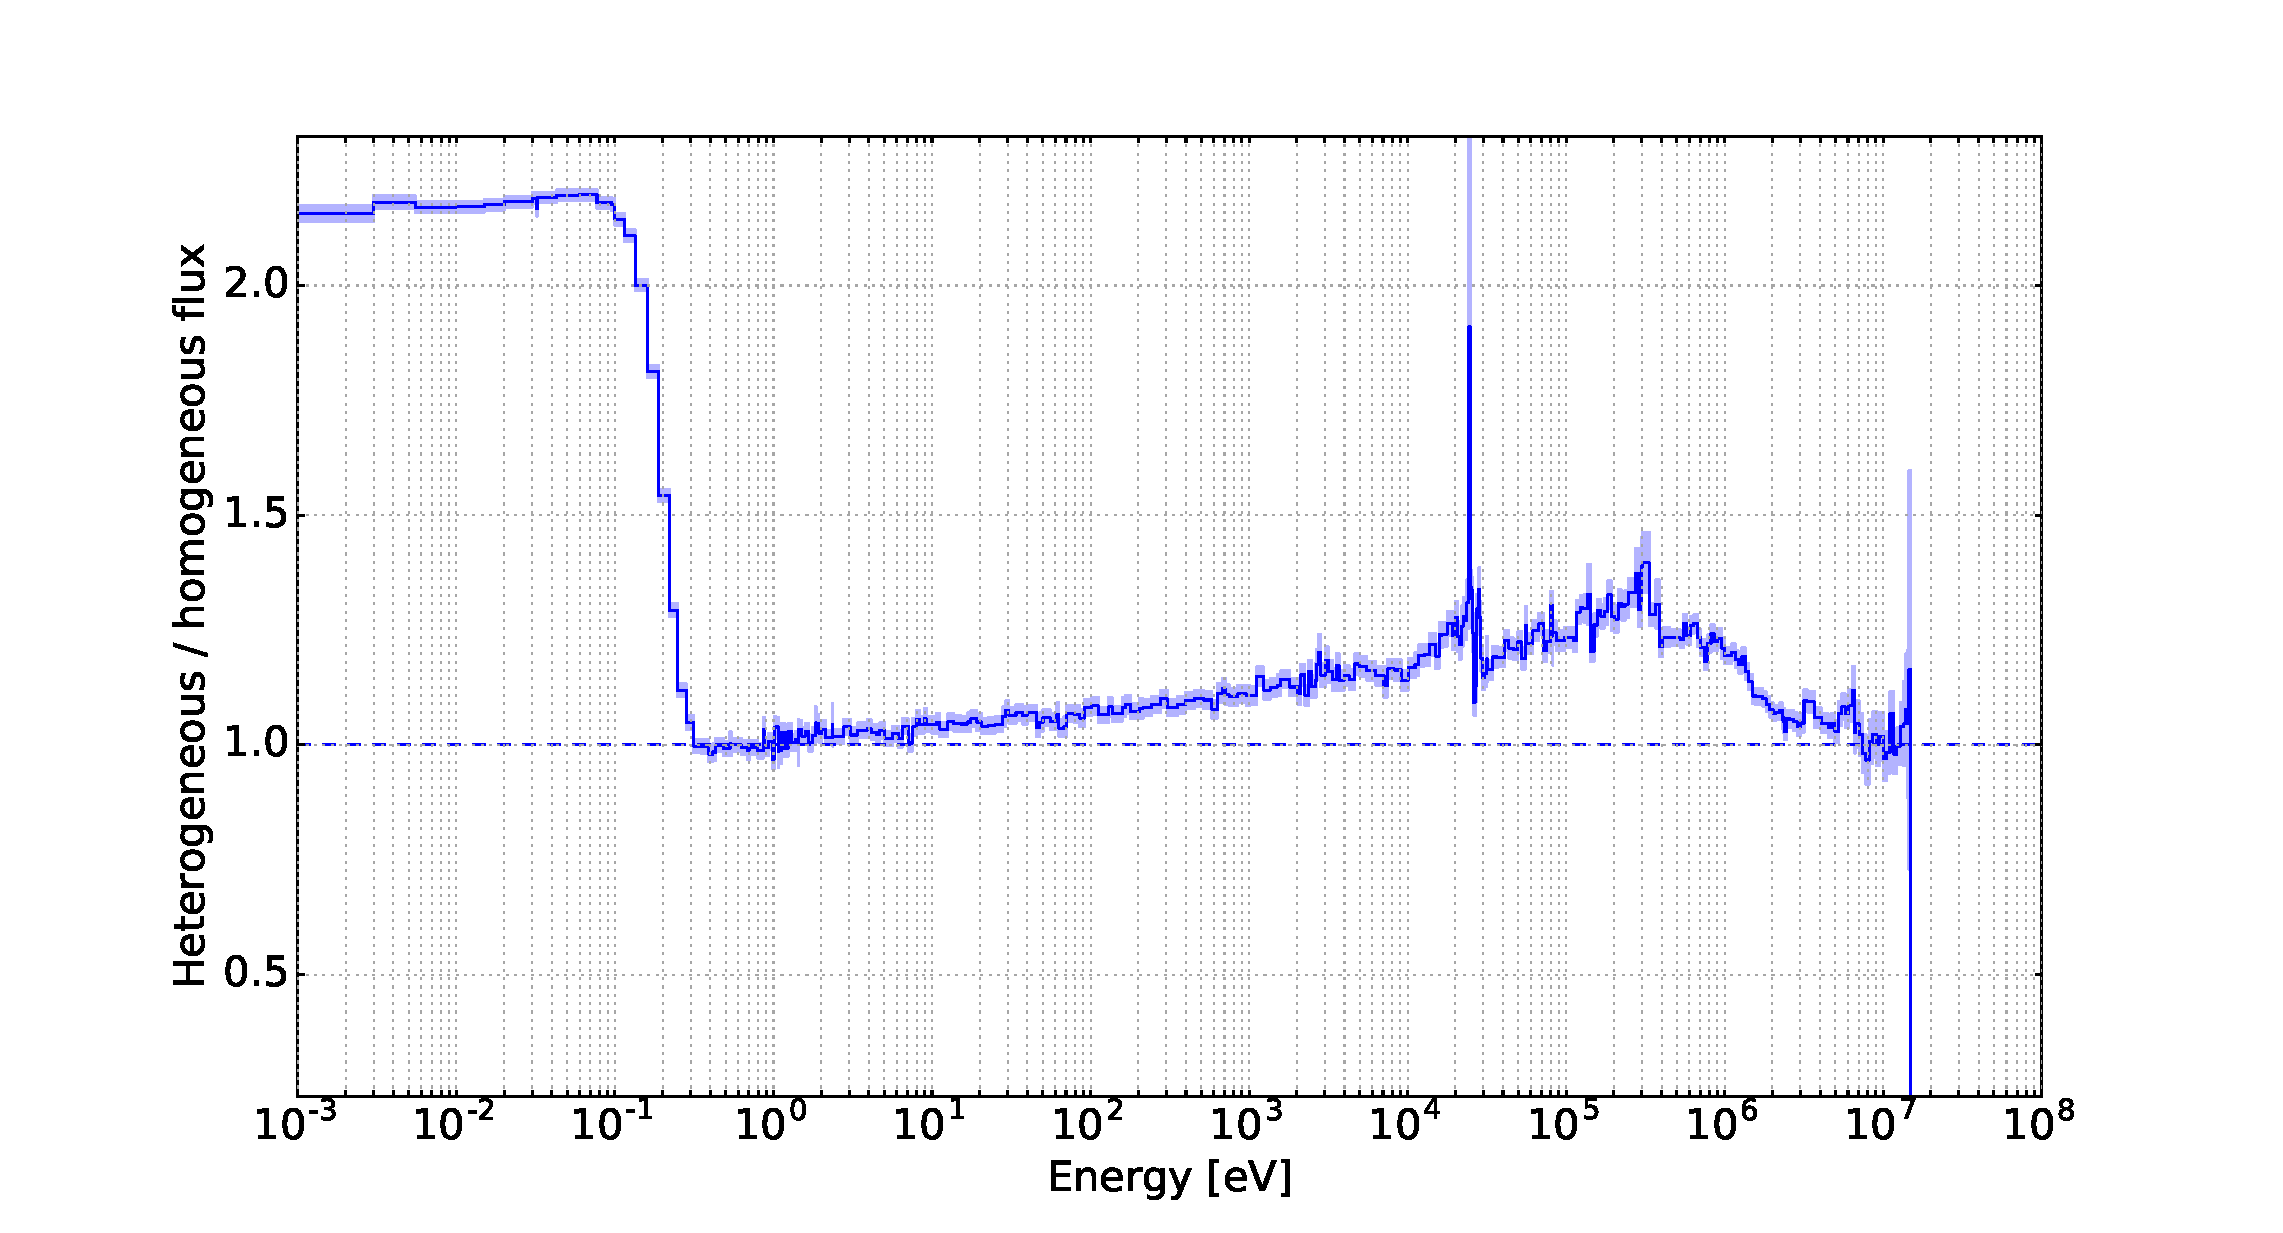
\includegraphics[width=\textwidth]{relative_neutron_spectra}
	\caption{The homogeneous flux increases are readily visible here.}
	\label{fig:relative_neutron_spectra}
\end{figure}

% % column span figure
% \begin{figure}[H]
%   \figuretitle{Contribution to neutron dose}
%   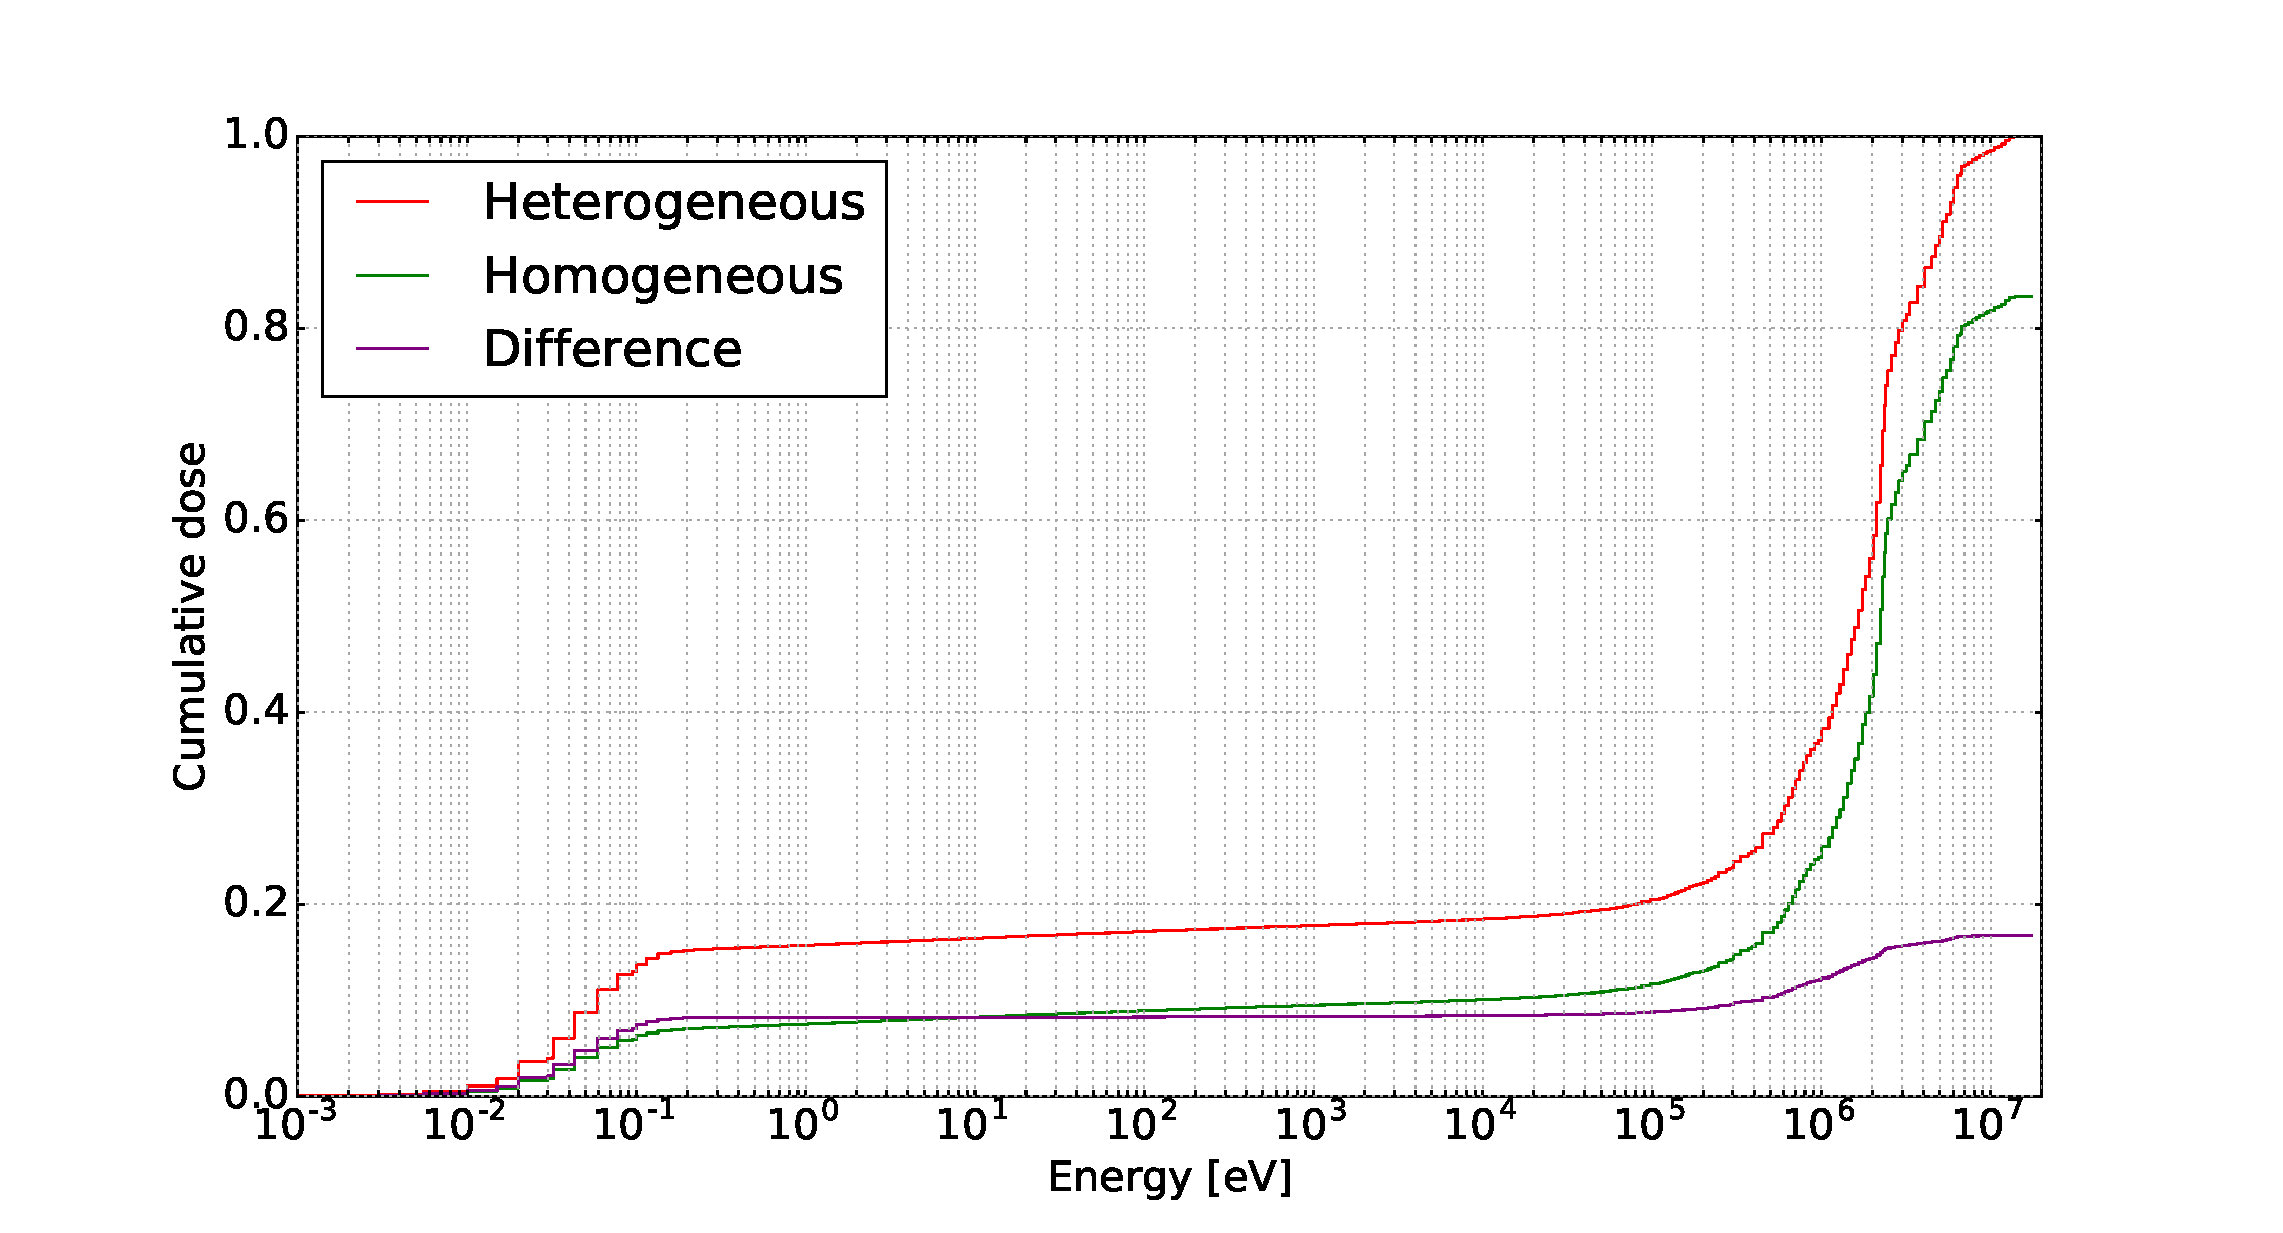
\includegraphics[width=0.5\textwidth]{cumulative_neutron_dose}
%   \caption{Here the dose is cumulatively summed along the energy axis, giving an indication of which energies the dose due to neutrons is from.}
%   \label{fig:cumulative_neutron_dose}
% \end{figure}

Figure \ref{fig:dose_discrepancy} shows how the discrepancy due to the homogeneous approximation varies with wall thickness. It can be seen that the effect is greatest for neutrons. It also plateaus at $\sim 1m$ wall thickness.

% column span figure
\begin{figure}[H]
  \figuretitle{Dose discrepancy due to homogeneity}
	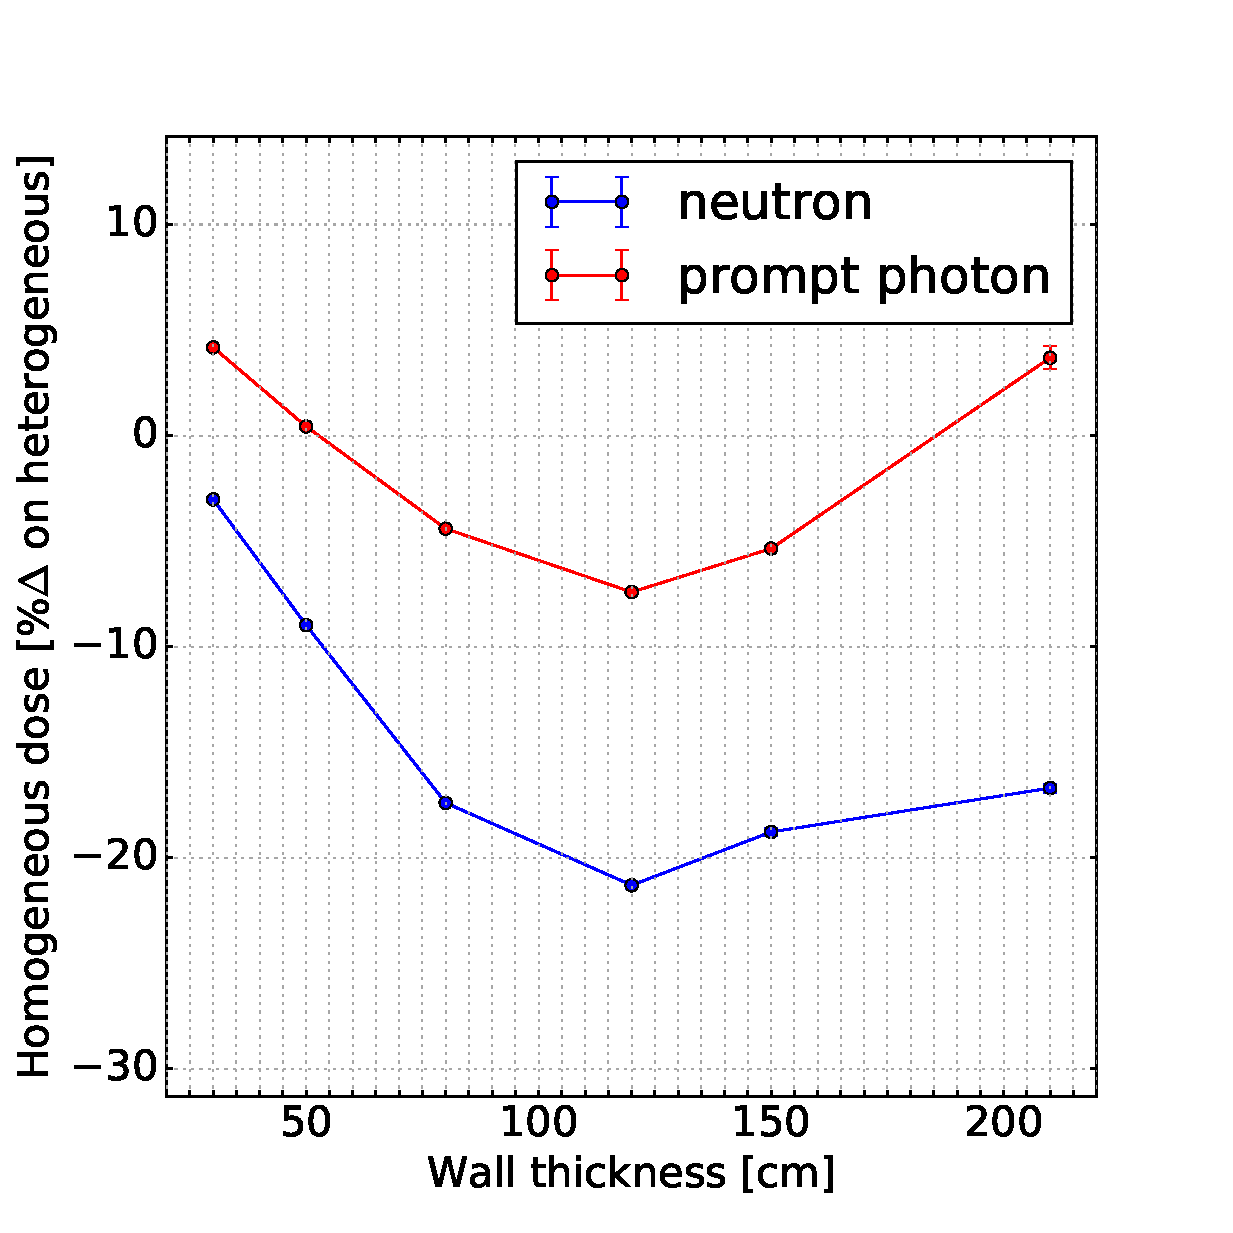
\includegraphics[width=\textwidth]{wall_thickness_dose_discrep}
	\caption{The discrepancy between modelling approaches is a function of the wall thickness for thin walls.}
	\label{fig:dose_discrepancy}
\end{figure}

\subsection{Shut Down Dose Rate}
\label{subsec:sddr}

After operation of a tokamak, repairs and maintenance are often necessary. This section explores the shut-down dose due to be received from the wall itself. It assumes a worker is inside the bioshield at ITER, stood 30cm from the inner surface of an activated wall.\par
Spatial homogenisation acts to overestimate the SDDR beyond 1 day (see figure \ref{fig:sddr}). The homogenised steel in the first few centimeters of the wall is activated by a stronger neutron flux than the physical rebar, located some 5--10cm inside the concrete (the cover depth).

% column span figure
\begin{figure}[H]
  \figuretitle{Shut-down $\phi_{\gamma}$ 30cm from irradiated concrete}
	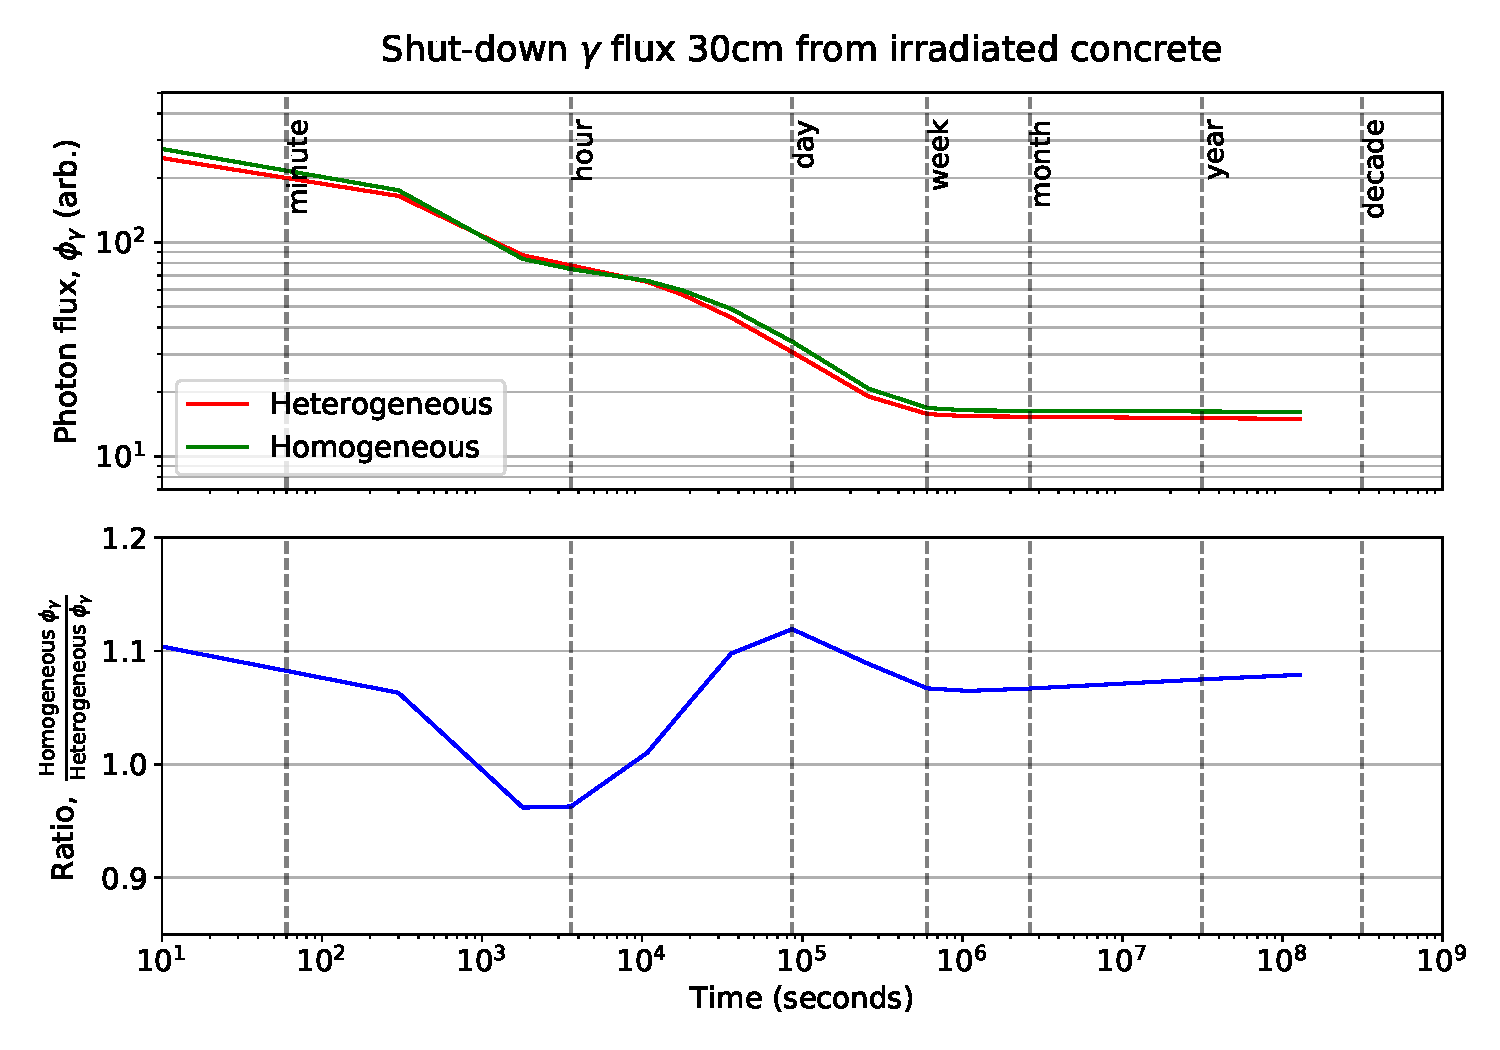
\includegraphics[width=\textwidth]{sddr}
	\caption{The total $\phi_{\gamma}$ as a function of cooling time. The homogeneous simulation gives a significantly increased value at time steps beyond $10^{5}s$ or approximately 1 day.}
	\label{fig:sddr}
\end{figure}

The mean free path of neutrons near the surface is $\sim2cm$ (see figure \ref{fig:mfp}) and as such a typical neutron will undergo several collisions before arriving at the rebar in a heterogeneous simulation. However, in a homogeneous simulation a small amount of steel is present right at the very surface of the concrete, as it is present throughout the simulation. This steel is exposed to an intense neutron flux and is activated accordingly.

% column span figure
\begin{figure}[H]
  \figuretitle{Neutron path length in concrete}
	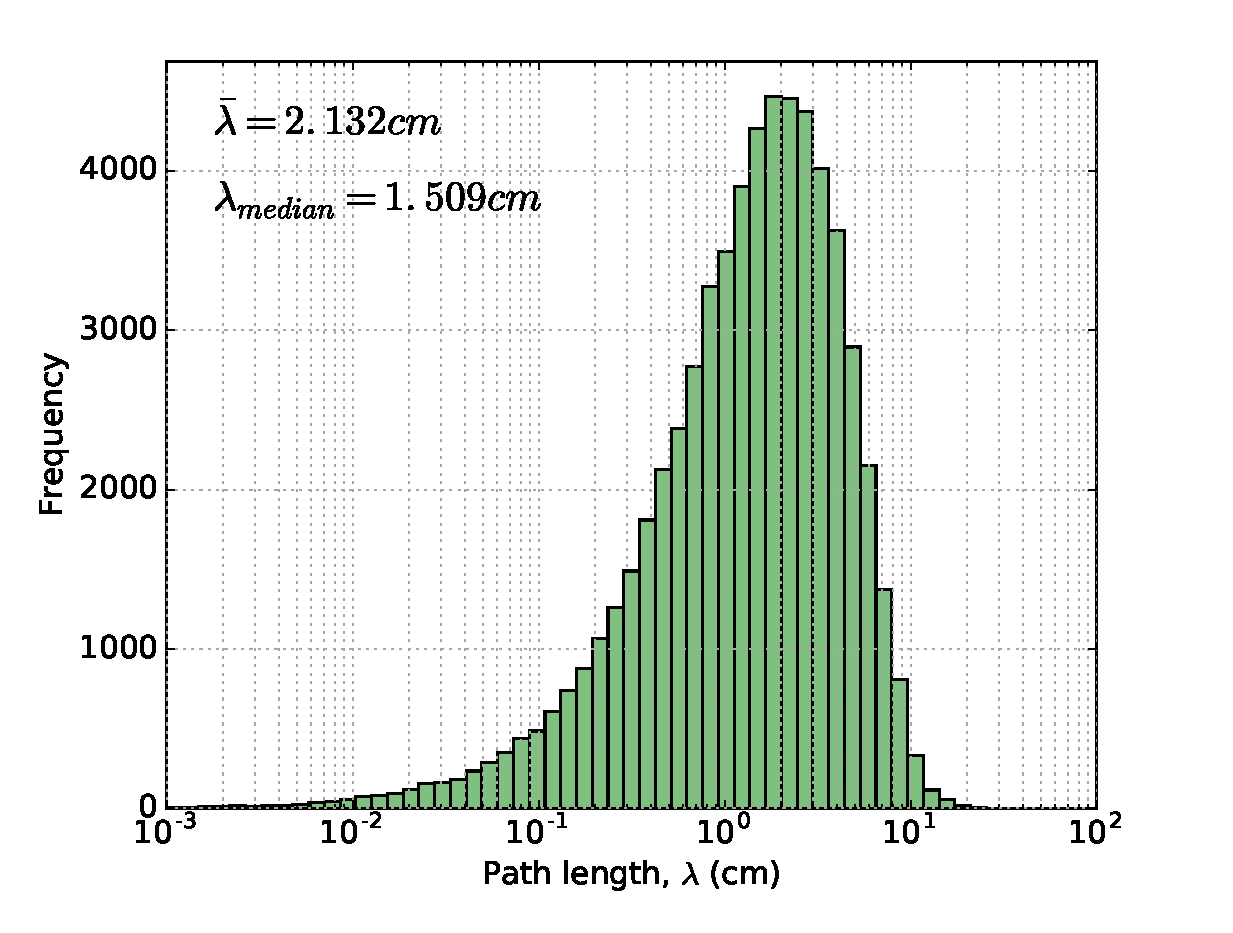
\includegraphics[width=\textwidth]{mfp}
	\caption{The path lengths of neutrons in pure concrete are shown as a histogram. There is a wide distribution with a mean of approximately 2cm.}
	\label{fig:mfp}
\end{figure}

The plot shown as figure \ref{fig:contact_dose} is produced with data from the activation solver FISPACT-II. Shown are estimates for a contact dose with concrete and steel. As the steel is buried within concrete, the numbers plotted here are not a substitute for transporting decay $\gamma$ photons from their birth to their death. However, they do give a good feel for which nuclides are responsible for the activity of a material at a given time. It is clear that after $^{28}$Al and $^{24}$Na decay in concrete, it has become substantially less active. It is around this time that steel becomes the dominant contributor to dose and the homogeneous modelling approach diverges from heterogeneous.

% column span figure
\begin{figure}[H]
  \figuretitle{Contact dose rate by material}
  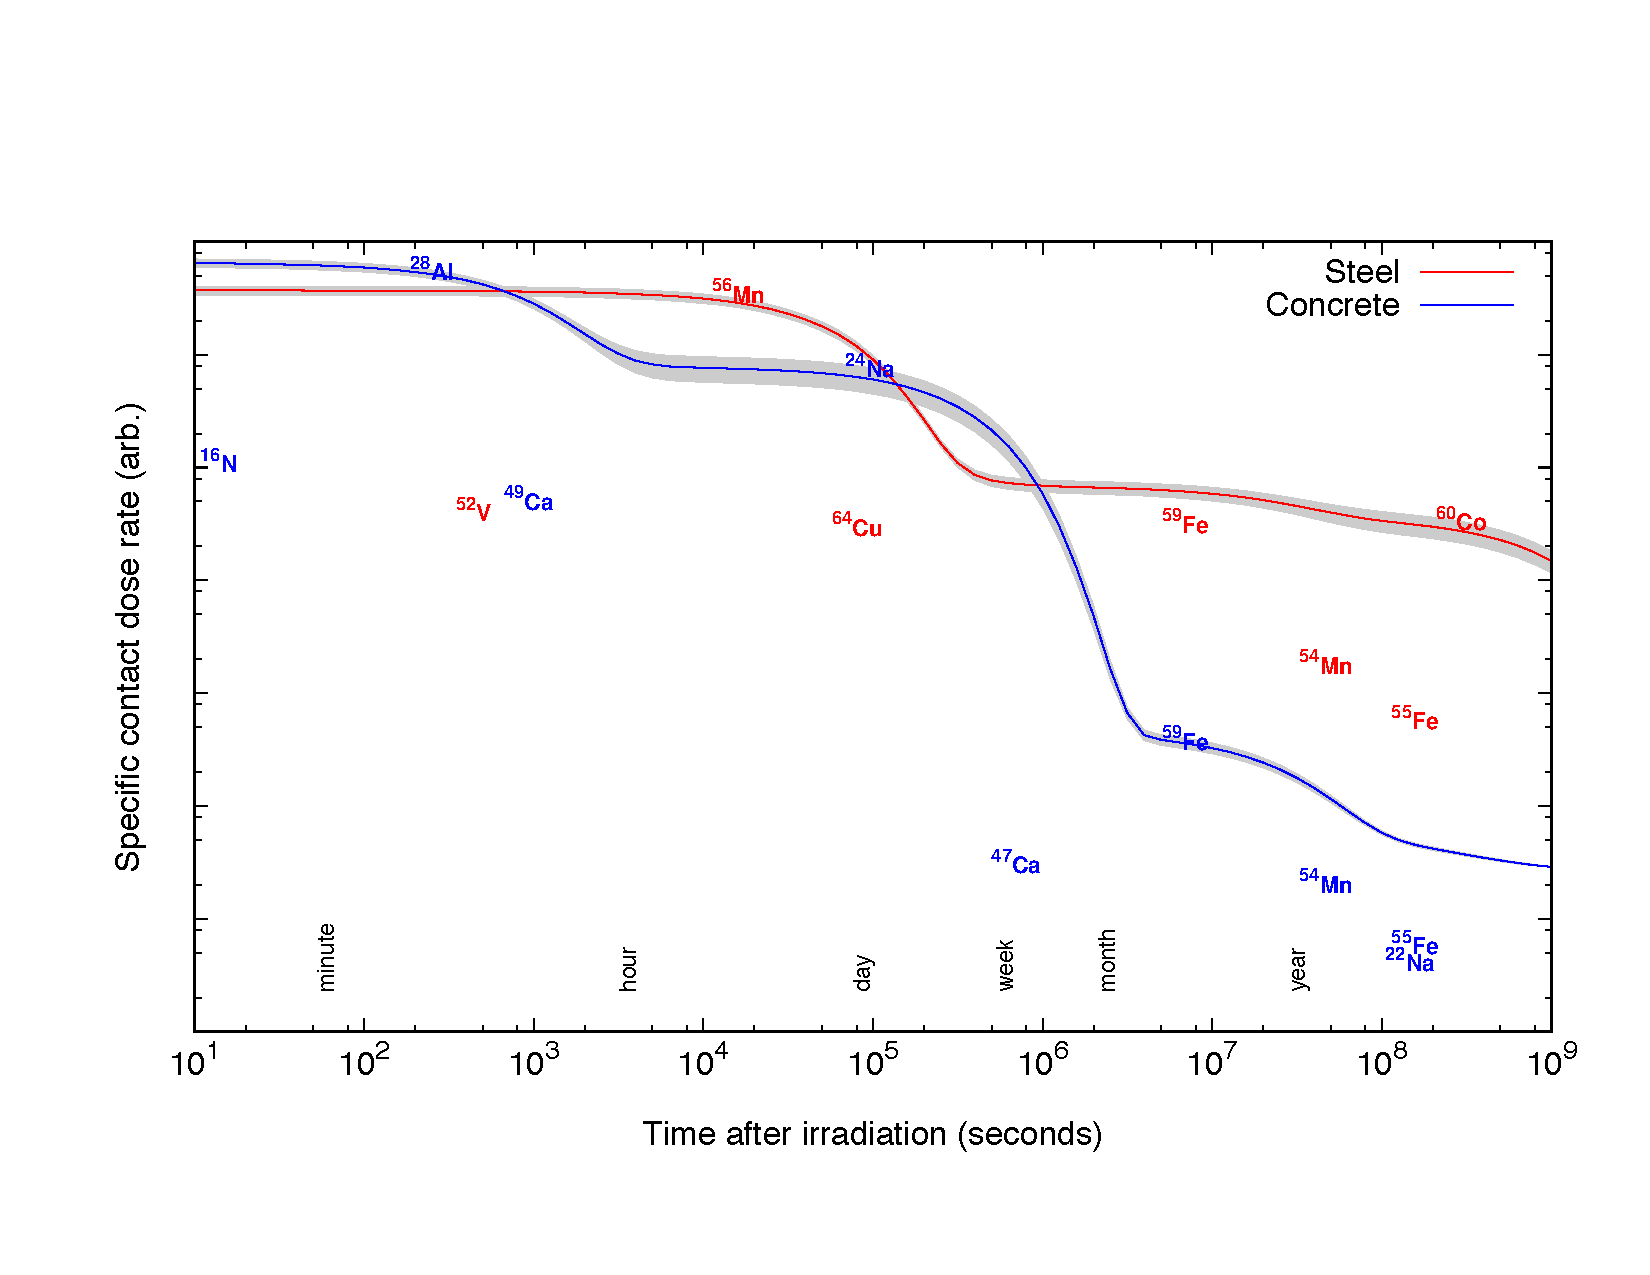
\includegraphics[width=\textwidth]{contact_dose_by_mat}
	\caption{This plot shows an estimate for the specific contact dose rate due to steel and concrete irradiated under the ITER SA-2 scenario. Nuclides which contribute a significant fraction of the dose are shown with their abscissa value as their half-life, $t_{\frac{1}{2}}$.}
	\label{fig:contact_dose}
\end{figure}

% % page span figure
% \end{multicols}
% \begin{figure}[H]
%   \begin{center}
%     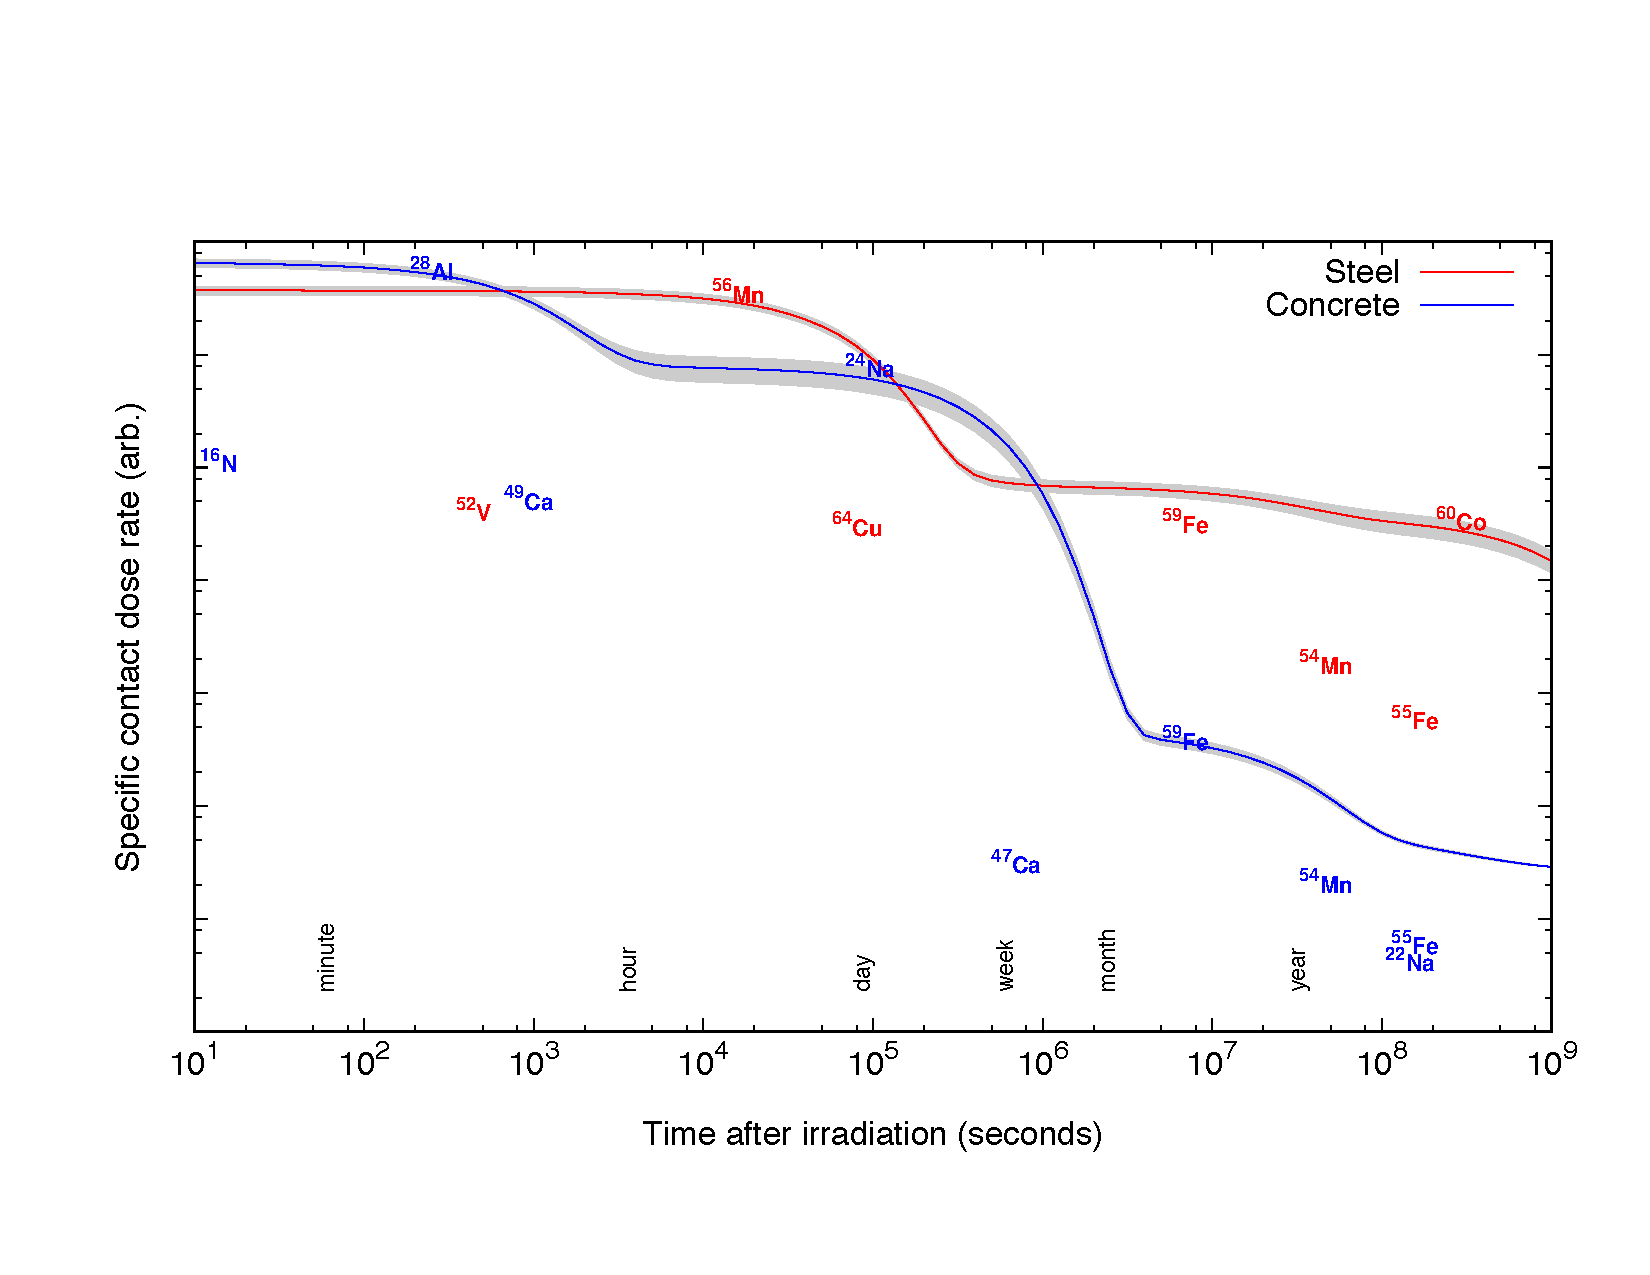
\includegraphics[width=0.8\textwidth]{contact_dose_by_mat}
%   \end{center}
%   \caption{This plot shows an estimate for the specific contact dose rate due to steel and concrete irradiated under the ITER SA-2 scenario. Nuclides which contribute a significant fraction of the dose are marked.}
%   \label{fig:contact_dose}
% \end{figure}
% \begin{multicols}{2}

\section{Conclusion}
The spatial homogenisation modelling approximation for reinforced concrete underestimates the dose due to neutrons by up to 20\%. The dose due to on-load photons can be underestimated by up to 8\%.\par
The SDDR is instead overestimated by homogenisation, by up to a factor 60 at times beyond a day. 
